\documentclass[a4paper,oneside,14pt]{extreport}

\usepackage[T2A]{fontenc}
\usepackage[utf8]{inputenc}
\usepackage[english,russian]{babel}

%\usepackage[left=30mm, right=20mm, top=20mm, bottom=20mm]{geometry}
\usepackage[left=20mm, right=10mm, top=5mm, bottom=20mm]{geometry}

\usepackage{microtype}
\sloppy

\usepackage{setspace}
\onehalfspacing

\usepackage{indentfirst}
\setlength{\parindent}{12.5mm}

\usepackage{titlesec}
\titleformat{\chapter}{\LARGE\bfseries}{\thechapter}{14pt}{\LARGE\bfseries}
\titlespacing*{\chapter}{\parindent}{0mm}{5mm}
\titleformat{\section}{\Large\bfseries}{\thesection}{14pt}{\Large\bfseries}

\addto{\captionsrussian}{\renewcommand*{\contentsname}{Содержание}}
\usepackage{natbib}
\renewcommand{\bibsection}{\chapter*{Список использованных источников}}

\usepackage{caption}

\usepackage{wrapfig}
\usepackage{float}

\usepackage{graphicx}
\newcommand{\imgwc}[4]
{
	\begin{figure}[#1]
		\center{\includegraphics[width=#2]{inc/img/#3}}
		\caption{#4}
		\label{img:#3}
	\end{figure}
}
\newcommand{\imghc}[4]
{
	\begin{figure}[#1]
		\center{\includegraphics[height=#2]{inc/img/#3}}
		\caption{#4}
		\label{img:#3}
	\end{figure}
}
\newcommand{\imgsc}[4]
{
	\begin{figure}[#1]
		\center{\includegraphics[scale=#2]{inc/img/#3}}
		\caption{#4}
		\label{img:#3}
	\end{figure}
}

\usepackage{pgfplots}
\pgfplotsset{compat=newest}

\usepackage{listings}
\usepackage{listingsutf8}
\lstset{
	basicstyle=\footnotesize\ttfamily,
	keywordstyle=\color{blue},
	stringstyle=\color{red},
	commentstyle=\color{gray},
	numbers=left,
	numberstyle=\tiny,
	numbersep=5pt,
	frame=false,
	breaklines=true,
	breakatwhitespace=true,
	inputencoding=utf8/koi8-r
}

\lstdefinestyle{c}{
	language=C++,
	backgroundcolor=\color{white},
	basicstyle=\footnotesize\ttfamily,
	keywordstyle=\color{blue},
	stringstyle=\color{red},
	commentstyle=\color{gray},
	directivestyle=\color{orange},
	numbers=left,
	numberstyle=\tiny,
	stepnumber=1,
	numbersep=5pt,
	frame=single,
	tabsize=4,
	captionpos=t,
	breaklines=true,
	breakatwhitespace=true,
	escapeinside={\#*}{*)},
	morecomment=[l][\color{magenta}]{\#},
	columns=fullflexible
}

\newcommand{\code}[1]{\texttt{#1}}

\usepackage{amsmath}
\usepackage{amssymb}

\usepackage[unicode]{hyperref}
\hypersetup{hidelinks}

\makeatletter
\newcommand{\vhrulefill}[1]
{
	\leavevmode\leaders\hrule\@height#1\hfill \kern\z@
}
\makeatother

\begin{document}
	
% ЗАДАНИЕ 2a Pinned Memory
\begin{figure}
	\begin{tikzpicture}
		\begin{axis}[
			xlabel={Размер матриц},
			ylabel={Время копирования, сек.},
			xtick={1000,2000,3000,4000,5000},
			legend pos=north west,
			ymajorgrids=true,
			grid style=dashed,
			width = 400
			]
			
			\addplot[
			color=blue,
			mark=square,
			]
			coordinates {
				(1000, 0.000497)(2000, 0.001767)(3000, 0.004237)(4000, 0.005760)(5000, 0.011798)
			};
			\addlegendentry{Pinned Memory}
			
			
			\addplot[
			color=green,
			mark=square,
			]
			coordinates {
				(1000, 0.000906)(2000, 0.003129)(3000, 0.007427)(4000, 0.013596)(5000, 0.021703)
			};
			\addlegendentry{Global Memory}
			
		\end{axis}
	\end{tikzpicture}
	\caption{Задание 2a - Зависимость времени копирования матриц от размера}
\end{figure}

% ЗАДАНИЕ 2c Cuda Streams
\begin{figure}
	\begin{tikzpicture}
		\begin{axis}[
			xlabel={Размер матриц},
			ylabel={Время копирования, сек.},
			xtick={1000,2000,3000,4000,5000},
			legend pos=north west,
			ymajorgrids=true,
			grid style=dashed,
			width = 400
			]
			
			\addplot[
			color=blue,
			mark=square,
			]
			coordinates {
				(1000, 0.001704)(2000, 0.005316)(3000, 0.010674)(4000, 0.018574)(5000, 0.028626)
			};
			\addlegendentry{Используя CUDA-потоки}
			
			
			\addplot[
			color=green,
			mark=square,
			]
			coordinates {
				(1000, 0.001734)(2000, 0.006809)(3000, 0.015014)(4000, 0.026589)(5000, 0.041031)	
			};
			\addlegendentry{Не используя CUDA-потоки}
			
		\end{axis}
	\end{tikzpicture}
	\caption{Задание 2c - Зависимость времени выполнения умножения матриц от размера матрицы}
\end{figure}

\begin{figure}
\begin{tikzpicture}
	\begin{axis}[
		xlabel={Размер матриц},
		ylabel={GFLOPS},
		xtick={1000,2000,3000,4000,5000},
		legend pos=north west,
		ymajorgrids=true,
		grid style=dashed,
		width = 400
		]
		
		\addplot[
		color=blue,
		mark=square,
		]
		coordinates {
			(1000, 1173.470981)(2000, 3009.553528)(3000, 5058.792779)(4000, 6891.532770)(5000, 8733.437306)
		};
		\addlegendentry{Используя CUDA-потоки}
		
		
		\addplot[
		color=green,
		mark=square,
		]
		coordinates {
			(1000, 1153.587789)(2000, 2349.804113)(3000, 3596.682260)(4000, 4814.096821)(5000, 6092.941455)
		};
		\addlegendentry{Не используя CUDA-потоки}
		
	\end{axis}
\end{tikzpicture}
\caption{Задание 2c - Зависимость GFLOPS умножения матриц от размера матрицы}
\end{figure}


% ЗАДАНИЕ 2d Shared Memory
\begin{figure}
	\begin{tikzpicture}
		\begin{axis}[
			xlabel={Размер матриц},
			ylabel={Время выполнения, сек.},
			xtick={500,1000,1500},
			legend pos=north west,
			ymajorgrids=true,
			grid style=dashed,
			width = 400
			]
			
			\addplot[
			color=blue,
			mark=square,
			]
			coordinates {
				(500, 0.000026)(1000, 0.000049)(1500, 0.000075)
			};
			\addlegendentry{Shared Memory}
			
			
			\addplot[
			color=green,
			mark=square,
			]
			coordinates {
				(500, 0.000035)(1000, 0.000069)(1500, 0.000103)
			};
			\addlegendentry{Global Memory}
			
		\end{axis}
	\end{tikzpicture}
	\caption{Задание 2d - Зависимость времени выполнения умножения матриц от размера матриц и типа памяти}
\end{figure}

\begin{figure}
	\begin{tikzpicture}
		\begin{axis}[
			xlabel={Размер матриц},
			ylabel={GFLOPS},
			xtick={500,1000,1500},
			legend pos=north west,
			ymajorgrids=true,
			grid style=dashed,
			width = 400
			]
			
			\addplot[
			color=blue,
			mark=square,
			]
			coordinates {
				(500, 9696.551900)(1000, 40422.257654)(1500, 89839.111370)
			};
			\addlegendentry{Shared Memory}
			
			
			\addplot[
			color=green,
			mark=square,
			]
			coordinates {
				(500, 7050.711242)(1000, 29009.695336)(1500, 65845.903011)
			};
			\addlegendentry{Global Memory}
			
		\end{axis}
	\end{tikzpicture}
	\caption{Задание 2d - Зависимость GFLOPS умножения матриц от размера матриц и типа памяти}
\end{figure}

% ЗАДАНИЕ 3 оптимизация Shared Memory
\begin{figure}
	\begin{tikzpicture}
		\begin{axis}[
			xlabel={Размер матриц},
			ylabel={Время выполнения, сек.},
			xtick={500,1000,1500},
			legend pos=north west,
			ymajorgrids=true,
			grid style=dashed,
			width = 400
			]
			
			\addplot[
			color=blue,
			mark=square,
			]
			coordinates {
				(500, 0.000015)(1000, 0.000027)(1500, 0.000040)
			};
			\addlegendentry{Shared Memory THREADS\_N = 16}
			
			
			\addplot[
			color=green,
			mark=square,
			]
			coordinates {
				(500, 0.000026)(1000, 0.000049)(1500, 0.000075)
			};
			\addlegendentry{Shared Memory THREADS\_N = 32}
			
		\end{axis}
	\end{tikzpicture}
	\caption{Задание 3 - Зависимость времени выполнения умножения матриц от размера матриц и оптимизации}
\end{figure}

\begin{figure}
\begin{tikzpicture}
	\begin{axis}[
		xlabel={Размер матриц},
		ylabel={GFLOPS},
		xtick={500,1000,1500},
		legend pos=north west,
		ymajorgrids=true,
		grid style=dashed,
		width = 400
		]
		
		\addplot[
		color=blue,
		mark=square,
		]
		coordinates {
			(500, 17006.340218)(1000, 73903.335664)(1500, 168185.412738)
		};
		\addlegendentry{Shared Memory THREADS\_N = 16}
		
		
		\addplot[
		color=green,
		mark=square,
		]
		coordinates {
			(500, 9696.551900)(1000, 40422.257654)(1500, 89839.111370)
		};
		\addlegendentry{Shared Memory THREADS\_N = 32}
		
	\end{axis}
\end{tikzpicture}
\caption{Задание 3 - Зависимость GFLOPS умножения матриц от размера матриц и оптимизации}
\end{figure}

% ЗАДАНИЕ 4-5 cuBlas openMP
\begin{figure}
	\begin{tikzpicture}
		\begin{axis}[
			xlabel={Размер матриц},
			ylabel={Время выполнения, сек.},
			xtick={500,1000,1500},
			legend pos=north west,
			ymajorgrids=true,
			grid style=dashed,
			width = 400
			]
			
			\addplot[
			color=blue,
			mark=square,
			]
			coordinates {
				(500, 0.000038)(1000, 0.000080)(1500, 0.000122)
			};
			\addlegendentry{Моя реализация}
			
			
			\addplot[
			color=green,
			mark=square,
			]
			coordinates {
				(500, 0.000029)(1000, 0.000171)(1500, 0.000556)
			};
			\addlegendentry{Библиотека CuBlas}
			
			\addplot[
			color=red,
			mark=square,
			]
			coordinates {
				(500, 0.001916)(1000, 0.011163)(1500, 0.041715)
			};
			\addlegendentry{OpenMP}
			
		\end{axis}
	\end{tikzpicture}
	\caption{Задания 4 и 5 - Зависимость времени выполнения умножения матриц от размера матриц и используемой библиотеки}
\end{figure}

\begin{figure}
	\begin{tikzpicture}
		\begin{axis}[
			xlabel={Размер матриц},
			ylabel={GFLOPS},
			xtick={500,1000,1500},
			legend pos=north west,
			ymajorgrids=true,
			grid style=dashed,
			width = 400
			]
			
			\addplot[
			color=blue,
			mark=square,
			]
			coordinates {
				(500, 6513.912684)(1000, 25041.407868)(1500, 55520.037230)
			};
			\addlegendentry{Моя реализация}
			
			
			\addplot[
			color=green,
			mark=square,
			]
			coordinates {
				(500, 8723.436088)(1000, 11675.251428)(1500, 12138.911241)
			};
			\addlegendentry{Библиотека CuBlas}
			
			\addplot[
			color=red,
			mark=square,
			]
			coordinates {
				(500, 130.473453)(1000, 179.160306)(1500, 161.811457)
			};
			\addlegendentry{OpenMP}
			
		\end{axis}
	\end{tikzpicture}
	\caption{Задания 4 и 5 - Зависимость GFLOPS умножения матриц от размера матриц и используемой библиотеки}
\end{figure}

% Задание 6 Profile Shared Memory
\begin{figure}[!h]
	\center{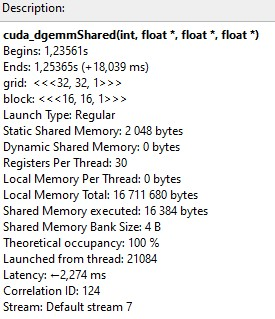
\includegraphics[width=1\linewidth]{task6}}
	\caption{Результат профилирование с помощью NVIDIA Nsight}
	\label{task6}
\end{figure}

\end{document}